\chapter{Transformada de Fourier}

% \section{Definiciones}

En el capítulo anterior, aprendimos que la serie de Fourier de $f \in \mathscr{C}[-L/2,L/2]$ está dada por 
\begin{equation} \label{Transformada1}
  f(x) = \sum_{n=-\infty}^{\infty} c_n e^{i \frac{2n\pi}{L}x} \ ,  
\end{equation}
donde 
\begin{equation} \label{Transformada2}
  c_n = \frac{1}{L} \int_{-L/2}^{L/2} f(x) e^{-i\frac{2n\pi}{L}x} \,dx, \quad n \in \mathbb{Z} \ . 
\end{equation}

Una consecuencia inmediata de la expansión en serie de Fourier es que la función $f(x)$ representada por la serie resulta periódica, con período $L$. Por lo tanto, decimos que la serie de Fourier permite \emph{expandir funciones periódicas}. 

Sin embargo, no todas las funciones son periódicas, y nos interesará expandirlas dentro de algún intervalo de validez. Necesitamos, entonces, algún modo de expandir, en una base ortonormal, funciones no periódicas. 

Podemos decir que el conjunto de coeficientes $\{c_n\}$ también definen a $f(x)$. Este conjunto de números $c_n$ puede ser entendido como una función en la variable $n$, escrita como $c(n)$, definida para un conjunto \emph{discreto} de valores de la variable independiente (en lugar de un intervalo continuo).  
\begin{defi}\marginnote{Espectro de Fourier}
    Se define como el \textbf{espectro de Fourier} a la función de variable discreta $c(n)$, definida a partir de los coeficientes de Fourier \eqref{Transformada2}.
\end{defi}

El espectro de una función puede ser graficado, asumiendo $c(n)$ real, como se observa en la figura \ref{fig:espectro-fourier}.

\vspace{-0.5cm}
\begin{figure}[H]
    \centering
    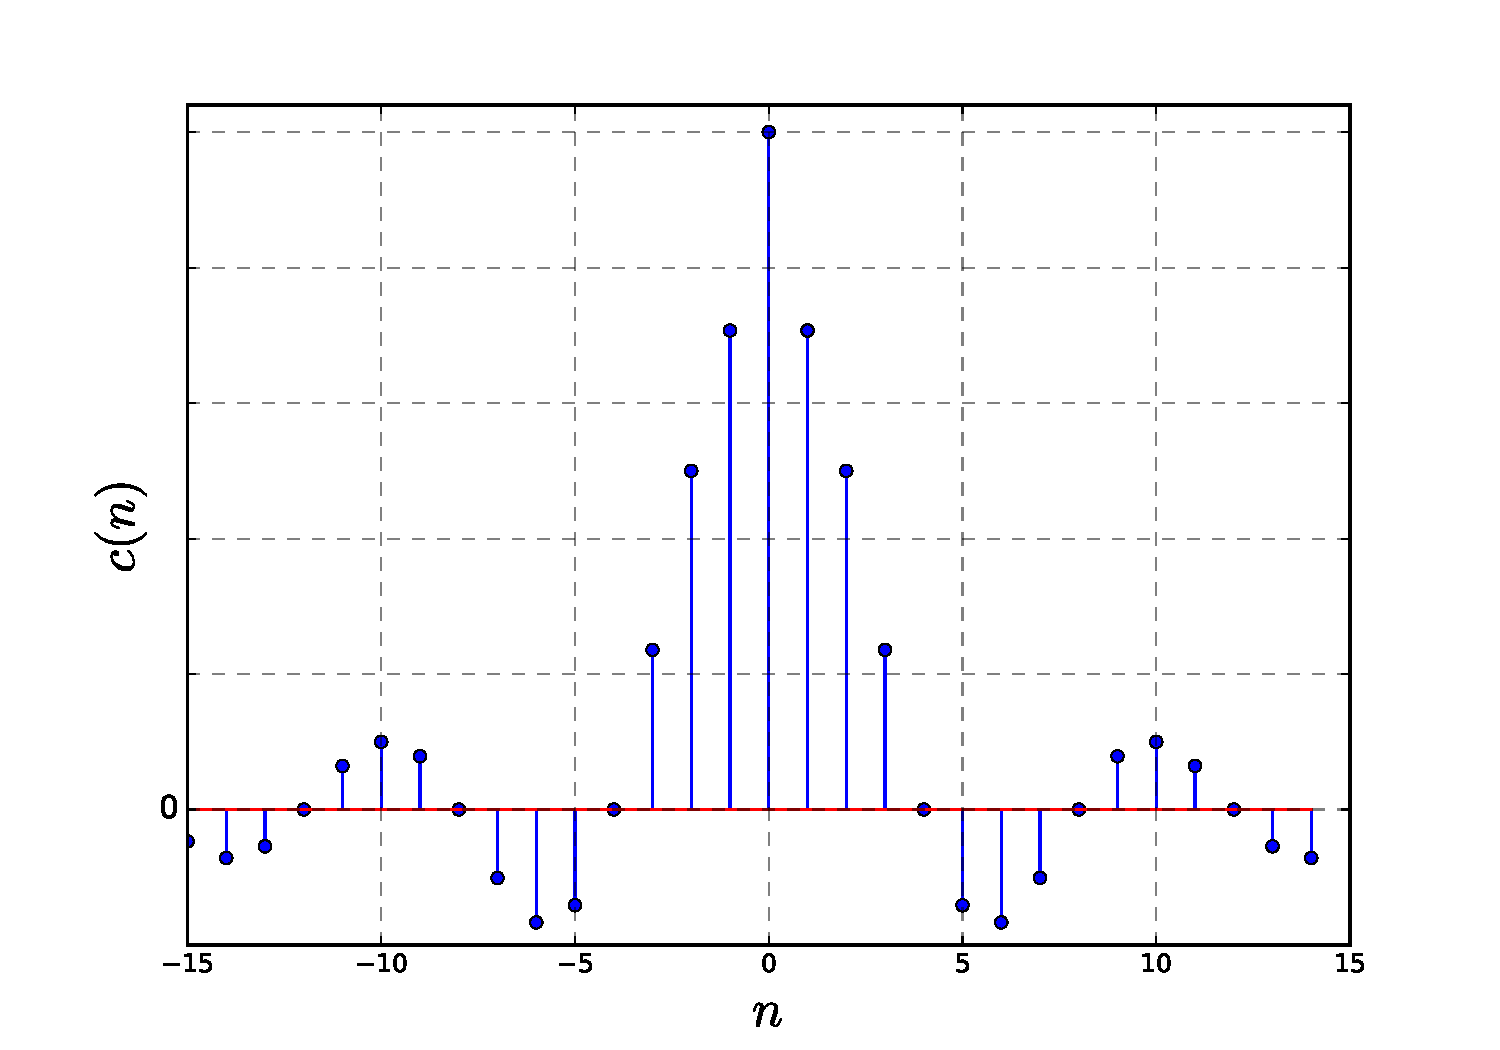
\includegraphics[width = 12cm]{Figuras/Espectro1.pdf}
    \caption{Espectro de Fourier.}
    \label{fig:espectro-fourier}
\end{figure}

En lugar de graficar $c$ vs $n$, podemos graficar $c$ vs $k$, el \emph{número de onda}, que corresponde a la frecuencia asociada a la parte espacial:
$$k = \frac{2\pi n}{L}.$$

Si $L \to \infty$, entonces las frecuencias se encuentran estrechamente espaciadas debido a que la diferencia entre valores consecutivos de $k$ es
$$\Delta k = \frac{ 2\pi \Delta n}{L}  = \frac{2\pi}{L}, \quad \mbox{pues}~ \Delta n = 1.$$

En otras palabras, para $L \to \infty$, $\Delta k$ es pequeño. Con este cambio de escala, el espectro de Fourier puede parecerse a lo mostrado en la figura \ref{Espectro1}.

\begin{figure}
    \centering
    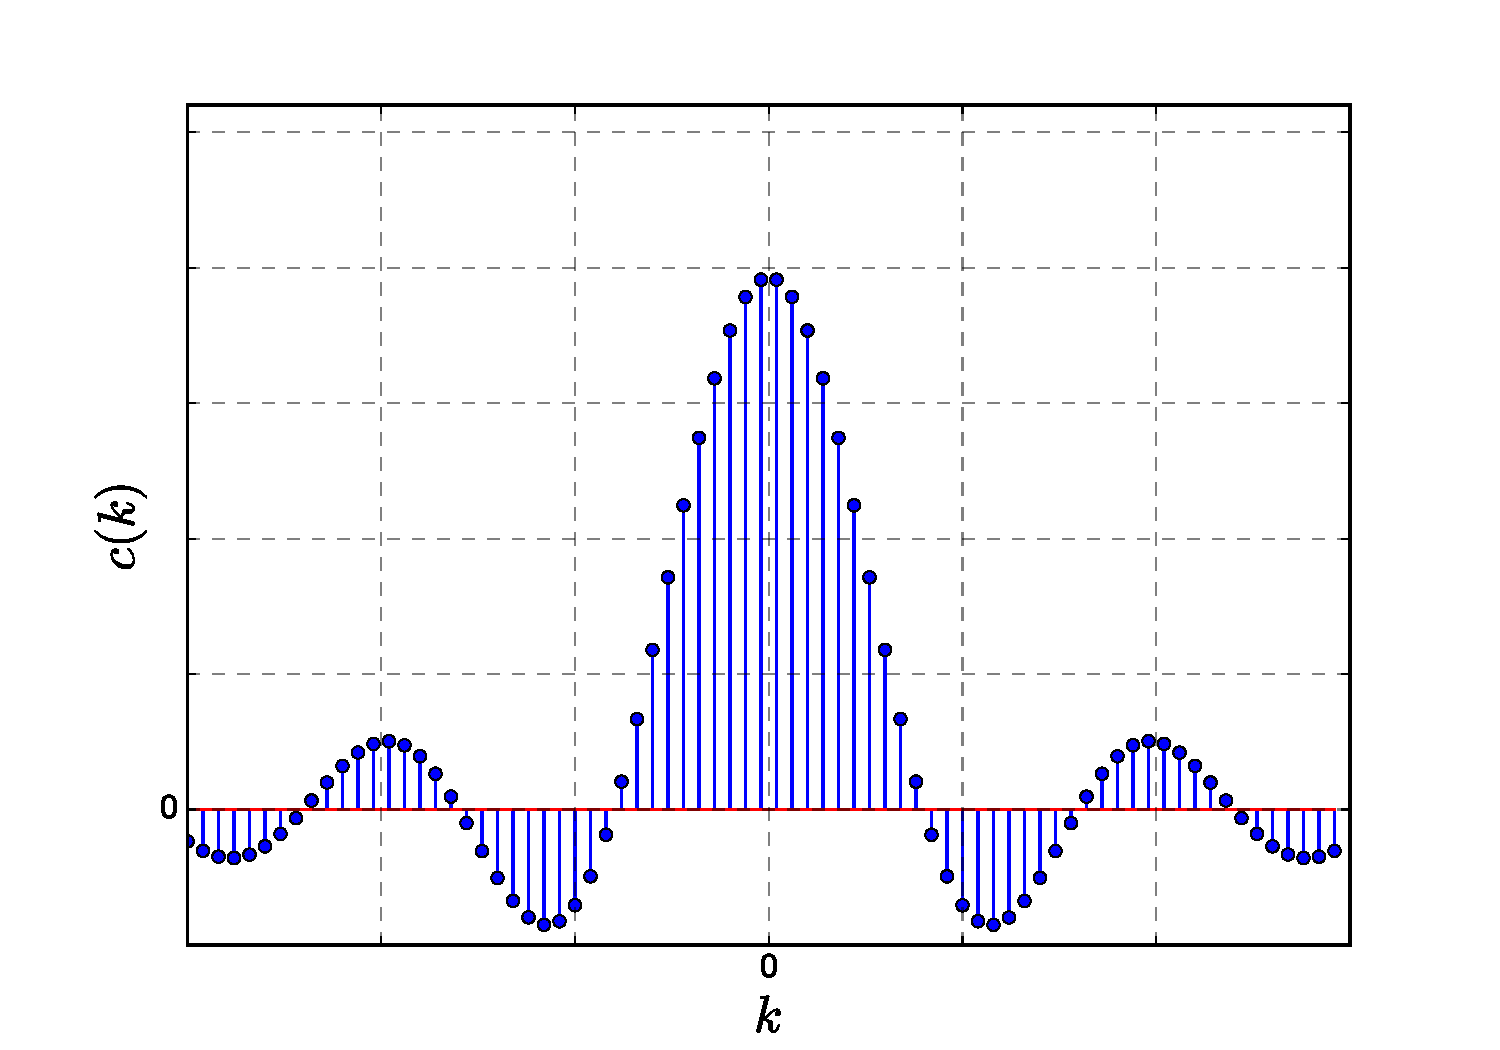
\includegraphics[scale = 0.4]{Figuras/Espectro2.pdf}
    \caption{Espectro de Fourier cuando $L \to + \infty$.}
    \label{Espectro1}
\end{figure}

Es natural especular sobre la posibilidad de un espectro continuo cuando $L$ tiende al infinito  de tal forma que todas las frecuencias están presentes. Puede ser instructivo considerar la siguiente derivación heurística: Sabemos que una función puede ser expandida como una serie de Fourier tal como se muestra en \eqref{Transformada1}. Luego, la transición $L \to \infty$ puede resultar difícil de realizar directamente ya que $c_n$ aparentemente tiende a cero. Seguimos entonces la idea de usar las frecuencias $k = 2\pi n/L$ tal que
$\Delta k = (2\pi/L ) \Delta n = 2\pi/L$ para valores de $k$ adyacentes y definimos
\begin{equation}
    c_L(k) = \frac{L}{\sqrt{2 \pi}} c_n \ .
\end{equation}

Usando las definiciones anteriores en las ecuaciones \eqref{Transformada1} y \eqref{Transformada2}, obtenemos que la función y sus coeficientes de Fourier se pueden escribir como: 
\begin{align*}
    f(x)&= \sum_{Lk/2\pi = -\infty}^{\infty} \frac{\sqrt{2\pi}}{L} c_L(k) e^{ikx} \left( \frac{\Delta k L}{2\pi}\right) = \sum_{Lk/2\pi = -\infty}^{\infty}  \frac{1}{\sqrt{2\pi}} c_L(k) e^{ikx} \Delta k , \\
  c_L(k) &= \frac{L}{\sqrt{2\pi}} \frac{1}{L} \int_{-L/2}^{L/2} f(x) e^{-ikx} dx = \frac{1}{\sqrt{2\pi}} \int_{-L/2}^{L/2} f(x) e^{-ikx} dx.
\end{align*}

Al hacer $L \to \infty$, la función $f$ puede considerarse como una función no-periódica arbitraria definida en todo el intervalo $(-\infty, \infty)$, mientras que la primera suma ``se convierte'' en una integral:
\begin{align*}
    f(x)& = \frac{1}{\sqrt{2\pi}} \int_{-\infty}^{\infty} c(k) e^{ikx} \,dk, \\
  c(k) & = \lim_{L\to + \infty} c_L(k) = \frac{1}{\sqrt{2\pi}} \int_{-\infty}^{\infty} f(x) e^{-ikx} dx.
\end{align*}

\begin{defi} \marginnote{Transformada de Fourier}
    Dada una función $f$ no periódica definida en $\mathscr{C}(-\infty, \infty)$, definimos su \textbf{transformada de Fourier} como 
    \begin{equation}\label{T.Fourier}
        \boxed{\tilde{f}(k) := \frac{1}{\sqrt{2\pi}} \int_{-\infty}^{\infty} f(x) e^{-ikx} dx \ .} 
    \end{equation}  
\end{defi}

Note que la transformada de Fourier es la extensión natural del concepto de series de Fourier para funciones no periódicas. Además, al ser $n$ una variable discreta, y $k$ continua, podemos decir que la transformada de Fourier es la generalización del concepto de series de Fourier cuando las funciones pertenecen a un espacio vectorial de dimensión continua.

\begin{defi}\marginnote{Transformada inversa de Fourier}
    Se define la \textbf{transformada inversa de Fourier} como
      \begin{equation}\label{I.Fourier}
     \boxed{f(x) = \frac{1}{\sqrt{2\pi}} \int_{-\infty}^{\infty} \tilde{f}(k) e^{ikx} \,dk \ .} 
    \end{equation}  
\end{defi}

\begin{obs}{Observaciones}
    \begin{itemize}
        \item Otras notaciones usadas son: $\tilde{f}(k) = \hat{f}(k) = g(k) = \mathcal{F}\{f(x)\}(k)$.
        
        \item El factor $1/\sqrt{2\pi}$ en la definición \eqref{T.Fourier} es convencional. Lo importante es que se cumpla la identidad conocida como \textbf{integral de Fourier}
        \begin{equation}
            f(x) = \int_{-\infty}^{\infty} \left[\frac{1}{2\pi} \int_{-\infty}^{\infty} f(\xi) e^{-ik\xi} d\xi \right] e^{ikx} \,dk.
          \label{IntegralFourier}
        \end{equation}
       
        % Por ejemplo, en lugar de estos factores, podría introducirse un $\alpha$ en \eqref{I.Fourier} y $1/(2\pi \alpha)$ en \eqref{T.Fourier}, con $\alpha$ una constante arbitraria. Algunas elecciones populares son: $\alpha = 1$ y $\alpha = 1/\sqrt{2\pi}$ \cite{Rubilar}.
    
        \item Al igual que el factor $1/\sqrt{2\pi}$ en la definición \eqref{T.Fourier}, la función $e^{-ikx}$ es convencional y puede ser reemplazada por $e^{ikx}$, siempre y cuando se verifique \eqref{IntegralFourier} \cite{Butkov, Riley}.
        
        % \item En el caso que $f(x)$ sea real, tenemos que \eqref{IntegralFourier} se puede escribir como 
        % \begin{equation}
        %     f(x) = \frac{1}{\pi} \int_{0}^{\infty} \int_{-\infty}^{\infty} f(\xi) \cos k(x-\xi)  \, d\xi \,dk.  \label{IntegralFourierReal}
        % \end{equation}
    
        % \colorlet{shadecolor}{blue!10} 
        % \begin{shaded}
        % En efecto, la relación \eqref{IntegralFourier} también se puede expresar como 
        % $$f(x) = \frac{1}{2\pi}  \int_{-\infty}^{\infty} \int_{-\infty}^{\infty} f(\xi) e^{-ik\xi} e^{ikx} d\xi  \,dk = \frac{1}{2\pi}  \int_{-\infty}^{\infty} \int_{-\infty}^{\infty} f(\xi) e^{ik(x-\xi)} d\xi  \,dk.$$
        
        % Como $f(x)$ es real, se igualan las partes reales para así obtener
        % $$f(x) = \frac{1}{2\pi} \int_{-\infty}^{\infty} \int_{-\infty}^{\infty} f(\xi) \cos k(x-\xi) d\xi  \,dk. $$
        
        % Puesto que $\cos k(x-\xi)$ es par con respecto a $k$, tenemos que 
        % $$f(x) = \frac{2}{2\pi} \int_{0}^{\infty} \int_{-\infty}^{\infty} f(\xi) \cos k(x-\xi)  \, d\xi \,dk =\frac{1}{\pi} \int_{0}^{\infty} \int_{-\infty}^{\infty} f(\xi) \cos k(x-\xi)  \, d\xi \,dk. $$  
        % \end{shaded}
        % \colorlet{shadecolor}{green!20}
        
        \item Es común en Física trabajar con funciones del tiempo, $f = f(t)$. En este caso, se acostumbra usar la frecuencia $\omega$ en lugar del número de onda $k$, de modo que la transformada de Fourier adopta la forma
        $$
        f(t) = \frac{1}{\sqrt{2\pi}} \int_{- \infty}^{\infty} \Tilde{f}(\omega) e^{i \omega t} d\omega,
        $$
    
        donde
        $$
        \Tilde{f}(\omega) = \frac{1}{\sqrt{2\pi}} \int_{- \infty}^{\infty} f(t) e^{- i \omega t} dt.
        $$
        
        \item En 3 dimensiones, la integral de Fourier está dada por:
        \begin{align*}
             f(\vec{r}\,) &:= \frac{1}{(2\pi)^{3/2}} \int_{\mathbb{R}^3} \tilde{f}(\vec{k}) e^{i (\vec{k} \cdot \vec{r})} d^3k, \\
             \tilde{f}(\vec{k}\,) &:= \frac{1}{(2\pi)^{3/2}} \int_{\mathbb{R}^3} f(\vec{r}) e^{-i (\vec{k} \cdot \vec{r})} d^3x.
        \end{align*}
        
        En general, en $n$ dimensiones:
         \begin{align*}
             f(\vec{r}\,) &:= \frac{1}{(2\pi)^{n/2}} \int_{\mathbb{R}^n} \tilde{f}(\vec{k}) e^{i (\vec{k} \cdot \vec{r})} d^n k, \\
             \tilde{f}(\vec{k}\,) &:= \frac{1}{(2\pi)^{n/2}} \int_{\mathbb{R}^n} f(\vec{r}) e^{-i (\vec{k} \cdot \vec{r})} d^n x.
        \end{align*}
       
    \end{itemize}    
\end{obs}


% \textbf{Observaciones:}

¿Cómo aseguramos la existencia de la transformada de Fourier de una función? Para ello, necesitamos introducir el concepto de \emph{funciones absolutamente integrables}, tras lo cual podemos plantear el teorema de existencia de la transformada de Fourier.

\begin{defi} \marginnote{Función absolutamente integrable}
Si $f(x)$ es tal que 
$$\int_{-\infty}^{\infty} |f(x)| \,dx < \infty,$$

entonces se dice que $f \in  L^1$ o que es \textbf{absolutamente integrable}.
\end{defi}

\begin{teorema}
Si $f \in L^1$, entonces la transformada de Fourier $\tilde{f}(k) = \mathcal{F}\{f(x)\}(k)$ existe y $\lim\limits_{k \to \pm \infty} \tilde{f}(k) = 0$.
\end{teorema}

\begin{demo}

Demostraremos solo la primera parte del teorema.

Notemos que
$$e^{-ikx} = \cos(kx) - i \sin(kx) ~\Rightarrow~ |e^{-ikx}| = 1.$$

Luego,
$$ \int_{-\infty}^{\infty} |f(x) e^{-ikx}| dx =  \int_{- \infty}^{\infty} |f(x)| \,dx < \infty.$$

En consecuencia, $f(x) e^{-ikx}$ es absolutamente integrable y
$$\frac{1}{2\pi} \int_{-\infty}^{\infty} f(x) e^{-ikx} dx$$

es finita, es decir, $\tilde{f}(k)$ existe. 
\end{demo}

\begin{obs}{Observación}
    La condición de que $f$ sea absolutamente integrable es suficiente pero no necesaria para la existencia de la transformada de Fourier.
\end{obs}

\begin{teorema}
    Sea $f(x)$ una función seccionalmente continua en cada intervalo finito del eje $x$, y supongamos que es absolutamente integrable en $(-\infty, + \infty)$. Entonces la \textbf{integral de Fourier} satisface
\begin{equation}
    \frac{1}{\pi} \int_0^{+\infty} \int_{-\infty}^{+\infty} f(\xi) \cos k(\xi-x) \,d\xi dk = \frac{f(x^+) + f(x^-)}{2} \ ,    
\end{equation}
donde ambas derivadas laterales, $f'(x^+)$ y $f'(x^-)$, existen.
\end{teorema}

\begin{demo}
Consulte el cápitulo 6 <<Fourier Integrals and Applications>> en \cite{Brown}.
\end{demo}

% \section{Ejemplos}

\begin{ejemplo} \label{PulsoCuadrado}
    \textbf{Función pulso cuadrado.} Consideremos la función 
    \begin{equation*}
        f(x) = \left\{ \begin{array}{cl}
            1,& |x|<a  \\
            0,& |x|> a
        \end{array} \right. \ .
    \end{equation*}

    Su transformada de Fourier es 
    \begin{align}
        \tilde{f}(k) & = \frac{1}{\sqrt{2\pi}} \int_{-\infty}^{\infty} f(x) e^{-ikx} dx \nonumber \\
        & = \frac{1}{\sqrt{2\pi}}\int_{-a}^a (1)  e^{-ikx} dx \nonumber \\
        & = \frac{1}{\sqrt{2\pi}} \left[ - \frac{1}{ik} e^{-ikx} \right]_{-a}^a \nonumber\\
        & = \frac{1}{\sqrt{2\pi} i k} [e^{ika} - e^{-ika}] \nonumber\\
        & = \sqrt{\frac{2}{\pi}} \frac{\sin(ka)}{k} \ . \label{TransPulsoCuadrado}
    \end{align}

    \begin{figure}[H]
        \centering
        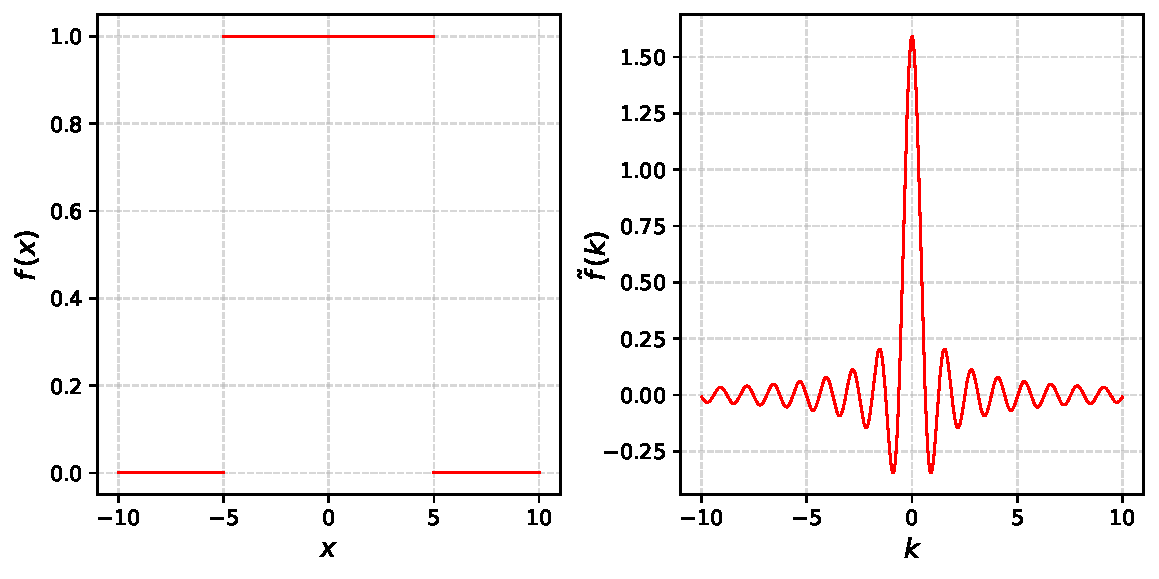
\includegraphics[scale = 0.55]{Figuras/EjemploTransformada1.pdf}
        \caption{Pulso cuadrado y su transformada de Fourier, con $a = 5$.}
        \label{Espectro2}
    \end{figure}

\end{ejemplo}

\begin{ejemplo}
    \textbf{Distribución gaussiana.} Considere la gaussiana
    \begin{equation*}
        f(x) = n e^{-\beta x^2}, \quad  \beta > 0 \ .
    \end{equation*}
    Su transformada de Fourier está dada por 
    \begin{equation*}
        \tilde{f}(k) =  \frac{n}{\sqrt{2\pi}} \int_{-\infty}^{\infty} e^{-\beta x^2} e^{-ikx} dx =  \frac{n}{\sqrt{2\pi}} \int_{-\infty}^{\infty} e^{-\beta x^2-ikx} dx .
    \end{equation*}

    Notemos que 
    \begin{align*}
        -\beta x^2-ikx &= - \beta \left( x^2 + \frac{ik}{\beta}x \right) \\
        &= - \beta \left( x^2 + \frac{ik}{\beta} x + \left( \frac{ik}{2\beta} \right)^2 - \left( \frac{ik}{2\beta} \right)^2 \right) \\
        &= - \beta \left( x + \frac{ik}{2\beta} \right)^2 + \beta \left( \frac{ik}{2\beta} \right)^2 \\
        &= - \beta \left( x + \frac{ik}{2\beta} \right)^2 - \left( \frac{k^2}{4\beta} \right).
    \end{align*}

    Luego, su transformada de Fourier puede escribirse como
    \begin{equation*}
        \tilde{f}(k) =  \frac{n}{\sqrt{2\pi}} \int_{-\infty}^{\infty} e^{-\beta \left( x + ik/2\beta \right)^2 - \left(k^2/4\beta \right)}  dx = \frac{n}{\sqrt{2\pi}} e^{- \left( k^2/4\beta \right)} \int_{-\infty}^{\infty} e^{-\beta \left( x + ik/2\beta \right)^2} \,dx. 
    \end{equation*}

    Haciendo el cambio de variable $u = x + \frac{ik}{2\beta}$, obtenemos que \footnote{}
    \begin{equation}\label{eq:Fourier-Gaussiana}
        \hat{f}(k) = \frac{n}{\sqrt{2\pi}} e^{- \left( k^2/4\beta \right)} \int_{-\infty}^{\infty} e^{-\beta u^2} \, du = \frac{n}{\sqrt{2\beta}} e^{- \left( k^2/4\beta \right)} \ ,
    \end{equation}
    donde hemos usado que 
    \begin{equation}
    \int_{-\infty}^{\infty} e^{-\beta x^2} \,dx = \sqrt{\frac{\pi}{\beta}}, \quad \beta > 0 \ . 
    \end{equation} 

    \begin{figure}[H]
        \centering
        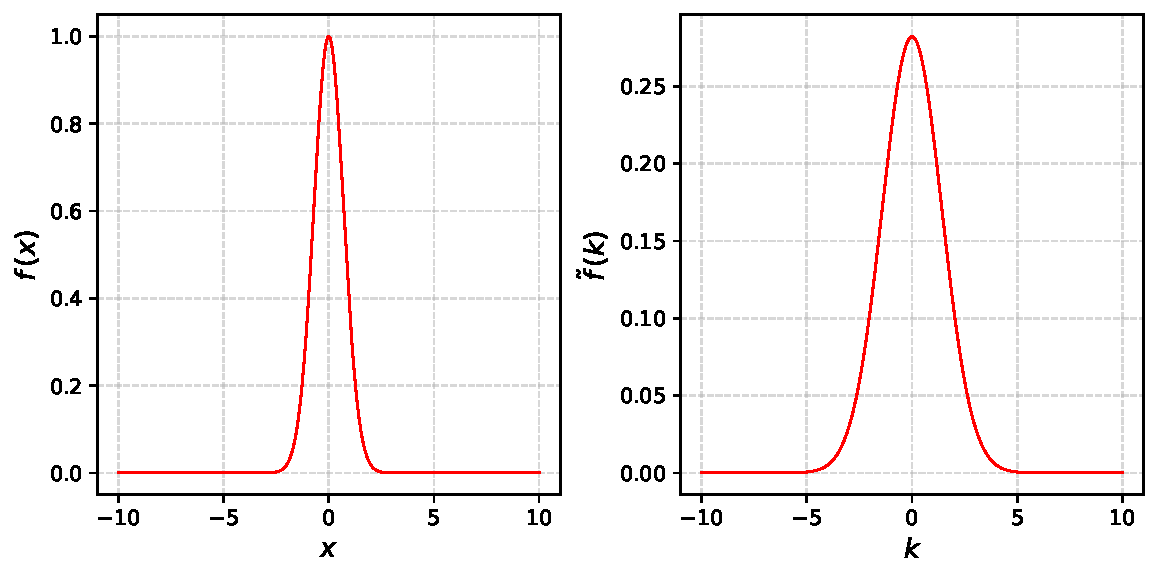
\includegraphics[width = 0.8\textwidth]{Figuras/EjemploTransformada2.pdf}
        \caption{Distribución gaussiana y su transformada de Fourier para $n=1$ y $\beta =1$ .}
        \label{Espectro3}
    \end{figure}
        \footnoterule
        
        {\footnotesize
        $^2$ En estricto rigor se debería calcular una integral compleja, vea \cite{Arfken}.
        }



    \begin{figure}[H]
        \centering
        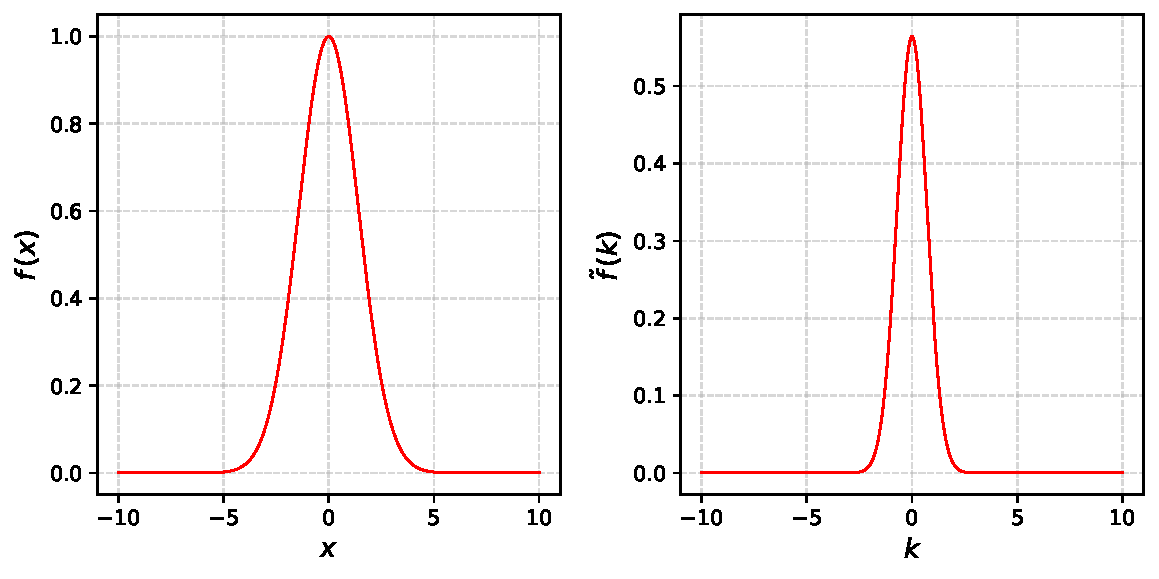
\includegraphics[scale = 0.6]{Figuras/EjemploTransformada3.pdf}
        \caption{Distribución gaussiana y su transformada de Fourier para $n=1$ y $\beta =0.25$ .}
        \label{Espectro4}
    \end{figure}
\end{ejemplo}


\section{Propiedades de la transformada de Fourier}

\begin{propiedad} 
\textbf{Propiedades de la Transformada de Fourier.} Sean las funciones $f, g \in L^1$ y los escalares $\alpha, \beta \in \mathbb{C}$.

\begin{enumerate}
    \item \textbf{Linealidad}: $$\mathcal{F}\{\alpha f(x) + \beta g(x)\}(k) = \alpha \mathcal{F}\{f(x)\}(k) + \beta \mathcal{F}\{g(x)\}(k).$$ 
    
    \item Si $f$ es real, entonces 
    % $$\tilde{f}(-k) = \tilde{f}^\ast(k).$$
    $$ \mathcal{F}\{f(x)\}(-k) = (\mathcal{F}\{f(x)\}(k))^*.$$
    
    \item \textbf{Traslación}: $$\mathcal{F}\{f(x+a)\}(k) = e^{ika} \mathcal{F}\{f(x)\}(k), \quad a \in \mathbb{R}.$$
    
    \item \textbf{Cambio de escala:} $$\mathcal{F}\{f(\alpha x)\}(k) = \frac{1}{|\alpha|}\mathcal{F}\{f(x)\}\left(\frac{k}{ \alpha}\right), \quad\alpha \neq 0.$$
    
    \item  \textbf{Atenuación}: $$\mathcal{F}\{f(x)e^{-ax}\}(k) =  \mathcal{F}\{f(x)\}(k-ia), \quad a \in \mathbb{C}.$$
    
    \item Si $f$ es una función par, entonces $\tilde{f}$ es una función real.
    
    \item Si $f$ es una función impar, entonces $\tilde{f}$ es una función puramente imaginaria, es decir, $\tilde{f}(k) = - \tilde{f}(-k)$.

    % \item \textbf{Escalonamiento:} $$\mathcal{F}\{f(\alpha x)\}(k) = \frac{1}{|\alpha|}\mathcal{F}\{f(x)\}\left(\frac{k}{ \alpha}\right), \quad\alpha \neq 0.$$
\end{enumerate}
\end{propiedad}

\begin{demo}
Demostraremos los puntos desde el 1 hasta el 5, y volveremos más tarde a los puntos 6 y 7.

\begin{enumerate}
    \item Por la definición \eqref{T.Fourier} de la transformada de Fourier y usando el hecho de que las funciones son absolutamente convergentes, tenemos
    \begin{align*}
        \mathcal{F}\{\alpha f(x) + \beta g(x)\}(k) &= \frac{1}{\sqrt{2\pi}} \int_{-\infty}^{\infty} [\alpha f(x) + \beta g(x)] e^{-ikx} dx \\
        &= \frac{\alpha}{\sqrt{2\pi}} \int_{-\infty}^{\infty}  f(x) e^{-ikx} dx + \frac{\beta}{\sqrt{2\pi}} \int_{-\infty}^{\infty}  g(x) e^{-ikx} dx \\
        &= \alpha \mathcal{F}\{f(x)\}(k) + \beta \mathcal{F}\{g(x)\}(k).
    \end{align*}
    
    \item Por la definición \eqref{T.Fourier} de la transformada de Fourier y suponiendo que $f$ es real:
    \begin{align*}
        \mathcal{F}\{f(x)\}(-k) &= \frac{1}{\sqrt{2\pi}} \int_{-\infty}^{\infty}  f(x)  e^{-(-ikx)} dx  \\
        &= \frac{1}{\sqrt{2\pi}} \int_{-\infty}^{\infty}  f(x)  (e^{-ikx})^* dx  \\
        &= \frac{1}{\sqrt{2\pi}} \int_{-\infty}^{\infty}  [f(x)  e^{-ikx}]^* dx \\
        &= (\mathcal{F}\{f(x)\}(k))^*.
    \end{align*}

    \item Por la definición \eqref{T.Fourier} de la transformada de Fourier, se tiene que
    \begin{equation*}
        \mathcal{F}\{f(x+a)\}(k) = \frac{1}{\sqrt{2\pi}}\int_{-\infty}^\infty f(x+a) e^{-ikx} dx \ .
    \end{equation*}

    Al hacer la sustitución $s = x+a$, $ds = dx$, tenemos
    \begin{align*}
        \frac{1}{\sqrt{2\pi}} \int_{-\infty}^\infty f(x+a)e^{-ikx}dx & = \frac{1}{\sqrt{2\pi}} \int_{-\infty}^\infty f(s) e^{-ik(s-a)} ds \\
        & = \frac{1}{\sqrt{2\pi}} \int_{-\infty}^\infty f(s) e^{-iks+ika} ds \\
        & = e^{ika} \left(\frac{1}{\sqrt{2\pi}} \int_{-\infty}^\infty e^{-iks} ds \right) \\
        & = e^{ika} \mathcal{F}\{f(x)\} (k) \ .
    \end{align*}

    \item Por la definición \eqref{T.Fourier} de la transformada de Fourier, se tiene que
    \begin{equation*}
        \mathcal{F} \{ f(\alpha x) \}(k) = \frac{1}{\sqrt{2\pi}} \int_{-\infty}^\infty f(\alpha x)e^{-ikx} dx \ .
    \end{equation*}

    Supondremos $\alpha > 0$. Haciendo el cambio de variable $u = \alpha x$, $du = \alpha dx$, tenemos
    \begin{equation*}
        \frac{1}{\sqrt{2\pi}} \int_{-\infty}^\infty f(\alpha x) e^{-ikx} dx = \frac{1}{\alpha} \left(\frac{1}{\sqrt{2\pi}} \int_{-\infty}^\infty f(u) e^{-i(k/\alpha)u} du \right) = \frac{1}{\alpha} \mathcal{F}\{f(x)\} \left( \frac{k}{\alpha} \right) \ .
    \end{equation*}

    Ahora, si $\alpha < 0$, hacemos el mismo cambio de variable que antes, obteniendo
    \begin{align*}
        \frac{1}{\sqrt{2\pi}} \int_{-\infty}^\infty f(\alpha x)e^{-ikx} dx & = \frac{1}{\alpha} \left( \frac{1}{\sqrt{2\pi}} \int_{\infty}^{-\infty} f(u) e^{-i(k/\alpha)u} du \right) \\ 
        & = - \frac{1}{\alpha} \left(\frac{1}{\sqrt{2\pi}} \int_{-\infty}^\infty f(u) e^{-i(k/\alpha)u} du \right) \\
        & = - \frac{1}{\alpha} \mathcal{F}\{f(x)\} \left(\frac{k}{\alpha}\right) \ .
    \end{align*}

    Por lo tanto, concluimos que, para $\alpha \neq 0$, se tendrá que
    \begin{equation*}
        \mathcal{F}\{(\alpha x)\}(k) = \frac{1}{|\alpha|} \mathcal{F}\{f(x)\} \left( \frac{k}{\alpha} \right) \ .
    \end{equation*}

    \item Por la definición \eqref{T.Fourier} de la transformada de Fourier, se tiene que
    \begin{align*}
        \mathcal{F}\{ f(x)e^{-ax} \}(k) & = \frac{1}{\sqrt{2\pi}} \int_{-\infty}^\infty f(x) e^{-ax} e^{-ikx} dx \\
        & = \frac{1}{\sqrt{2\pi}} \int_{-\infty}^\infty f(x) e^{-ikx-ax} dx \\
        & = \frac{1}{\sqrt{2\pi}} \int_{-\infty}^\infty f(x) e^{-ikx+i^2ax} dx \\
        & = \frac{1}{\sqrt{2\pi}} \int_{-\infty}^\infty e^{-ix(k-ia)} dx \\
        & = \mathcal{F}\{f(x)\}(k-ia) \ .
    \end{align*}
\end{enumerate}
\end{demo}

\begin{propo}\marginnote{Transformada de Fourier de una derivada}
Sea $f(x)$ con transformada de Fourier $\mathcal{F}\{f(x)\}$ y $\lim\limits_{x \to \pm \infty} f(x) = 0$. Entonces, 
\begin{equation}
    \boxed{\mathcal{F}\{f'(x)\} = i k \mathcal{F}\{f(x)\}\ ,} 
\end{equation}
y en general, 
\begin{equation}
    \mathcal{F}\{f^{(n)} (x)\} = (i k)^n \mathcal{F}\{f(x)\} \ ,
\end{equation}
\end{propo}

\begin{demo}
Demostraremos el caso para la primera derivada, pues derivadas más altas se deducen a partir de este. Usando la definición \eqref{T.Fourier} de la transformada de Fourier, tenemos que 
\begin{align*}
    \mathcal{F}\{f'(x)\} &= \frac{1}{\sqrt{2\pi}} \int_{- \infty}^{\infty} f'(x) e^{-ikx} \,dx \\
    &= \frac{1}{\sqrt{2\pi}} \int_{- \infty}^{\infty} \left\{ \frac{d}{dx}\left[ f(x) e^{-ikx} \right]  - (-ik) f(x) e^{-ikx} \right\}\,dx \\
    &= \frac{1}{\sqrt{2\pi}} \left. f(x) e^{-ikx} \right|_{-\infty}^{\infty} + \frac{ik}{\sqrt{2\pi}} \int_{- \infty}^{\infty}  f(x) e^{-ikx} \,dx \\
    &=  ik \mathcal{F}\{f(x)\} + \left. f(x) e^{-ikx} \right|_{-\infty}^{\infty}.
\end{align*}

Como  $\lim\limits_{x \to \pm \infty} f(x) = 0$, obtenemos
$$\mathcal{F}\{f'(x)\} = i k \mathcal{F}\{f(x)\}.$$
\end{demo}

% En general,
% \begin{shaded}
% $$,$$    
% \end{shaded}


Dado que hemos entendido la transformada de Fourier como una extensión de las series de Fourier, como es el caso de que las condiciones de existencia de la transformada de Fourier son las mismas \emph{condiciones de Dirichlet} para la existencia de los coeficientes de Fourier. Por ello, esperaríamos una analogía a la fórmula de Parseval propia de las series de Fourier. Esta corresponde al siguiente teorema.

\begin{teorema}[de Parseval]
Si $f(x)$ y $g(x)$ son funciones reales y si $\tilde{f}(k)$ y $\tilde{g}(k)$ son sus correspondientes transformadas de Fourier, entonces

\begin{itemize}
    \item[(i)] (Primer teorema)
    $$\int_{-\infty}^{\infty} |\tilde{f}(k)|^2\, dk = \int_{-\infty}^{\infty} |f(x)|^2 \, dx. $$
    
    \item[(ii)] (Segundo teorema)
    $$\int_{-\infty}^{\infty} \tilde{f}(k) \tilde{g}(-k) \, dk = \int_{-\infty}^{\infty} f(x) g(x) \, dx. $$
    
\end{itemize}
\end{teorema}

\begin{demo}
Notemos que (i) es consecuencia de (ii) al tomar $g(x) = f(x)$ real tal que $f^*(x) = f(x)$ y $\tilde{g}(-k) = \tilde{f}^*(k)$. Luego, nos bastará demostrar el segundo teorema de Parseval.

Usando la definición \eqref{T.Fourier}, tenemos que 
$$\tilde{g}(-k) = \frac{1}{\sqrt{2\pi}} \int_{-\infty}^{\infty} g(x) e^{ikx} \,dx.$$

Luego, 
$$\int_{-\infty}^{\infty} \tilde{f}(k) \tilde{g}(-k) \,dk = \int_{-\infty}^{\infty} \tilde{f}(k) \,dk \int_{-\infty}^{\infty} \frac{1}{\sqrt{2\pi}} g(x) e^{ikx} \,dx.$$

Supongamos que podemos intercambiar el orden de integración, por ejemplo, al suponer que las integrales 
$$\int_{-\infty}^{\infty} \tilde{f}(k) e^{ikx} \,dk ~~\mbox{y}~~ \int_{-\infty}^{\infty} g(x) e^{ikx} \,dx$$
son absolutamente integrables. Entonces,
$$\int_{-\infty}^{\infty} \tilde{f}(k) \tilde{g}(-k) \,dk = \int_{-\infty}^{\infty} g(x) \left( \frac{1}{\sqrt{2\pi}} \int_{-\infty}^{\infty} \tilde{f}(k) e^{ikx} \,dk\right) \,dx.$$

Aplicando la transformada inversa de Fourier dada por \eqref{I.Fourier}, concluimos que
$$\int_{-\infty}^{\infty} \tilde{f}(k) \tilde{g}(-k) \,dk = \int_{-\infty}^{\infty} f(x) g(x)  \,dx.$$

\end{demo}

\begin{ejemplo}
    Use el teorema de Parseval para evaluar
    $$\int_{-\infty}^{\infty}  \frac{\sin^2(x)}{x^2} \,dx.$$

    \textbf{Solución:} Esta integral puede ser calculada usando el teorema del residuo. En nuestro caso, usaremos el primer teorema de Parseval, teniendo en cuenta el resultado de la transformada de Fourier del pulso cuadrado en el ejemplo \ref{PulsoCuadrado}. 

    Para $a = 1$ en la ecuación \eqref{TransPulsoCuadrado}, tenemos que
    $$\int_{- \infty}^{\infty} |\Tilde{f}(k)|^2 \,dk = \int_{- \infty}^{\infty} \frac{2}{\pi} \frac{\sin^2(k)}{k^2}  \,dk = \frac{2}{\pi} \int_{-\infty}^{\infty}  \frac{\sin^2(k)}{k^2} \,dk.$$

    Por el primer teorema de Parseval,
    \begin{align*}
        \int_{- \infty}^{\infty} |\Tilde{f}(k)|^2 \,dk &= \int_{-\infty}^{\infty} |f(x)|^2 \,dx \\
        \Rightarrow \frac{2}{\pi} \int_{-\infty}^{\infty}  \frac{\sin^2(k)}{k^2} &=  \int_{-1}^1 \,dx = 2 \ . 
    \end{align*}

Por lo tanto,
$$\int_{-\infty}^{\infty}  \frac{\sin^2(k)}{k^2} \,dk = \pi.$$
\end{ejemplo}

\section{Transformadas seno y coseno}

Dependiendo de la paridad de las funciones a las cuales le aplicamos una transformada de Fourier, es posible utilizar una forma \emph{abreviada} de transformada, de manera similar a lo que podemos hacer para una serie de Fourier.

Notemos que, dada una función real $f(x)$ impar, tenemos que
\begin{align*}
    \tilde{f}(k) & = \frac{1}{\sqrt{2\pi}} \int_{-\infty}^{\infty} f(x) e^{-ikx} dx \\
    & = \frac{1}{\sqrt{2\pi}}  \int_{-\infty}^0 f(x) e^{-ikx} \,dx + \frac{1}{\sqrt{2\pi}} \int_{0}^{\infty} f(x) e^{-ikx} \, dx \\
    & = -\frac{1}{\sqrt{2\pi}}  \int_{\infty}^0 f(-x) e^{ikx} \,dx + \frac{1}{\sqrt{2\pi}}  \int_{0}^{\infty} f(x) e^{-ikx} \, dx \ , \quad x \to -x \mbox{ en la integral 1} \ , \\
    & = -\frac{1}{\sqrt{2\pi}} \int_{0}^{\infty} f(x) e^{ikx} \,dx + \frac{1}{\sqrt{2\pi}}  \int_{0}^{\infty} f(x) e^{-ikx} \, dx \ , \quad f(-x) = -f(x) \ ,  \\
     &= -\frac{1}{\sqrt{2\pi}}  \int_{0}^{\infty} f(x) [e^{ikx} - e^{-ikx}  ] \, dx \ , \quad \int_a^b = - \int_b^a \ , \\
    & = -\frac{2i}{\sqrt{2\pi}}  \int_{0}^{\infty} f(x) \sin(kx) \,dx \\
    & = -i \left(\sqrt{\frac{2}{\pi}}  \int_{0}^{\infty} f(x) \sin(kx) \,dx \right) \ .
    %  \equiv - i  \tilde{f}_S(k),
\end{align*}

\begin{defi}\marginnote{Transformada seno de Fourier}
    Se define la \textbf{transformada seno de Fourier}, $\tilde{f}_S(k) = \mathcal{F}_S(k)$ como
    \begin{equation}
        \tilde{f}_S(x) = \sqrt{\frac{2}{\pi}} \int_0^\infty f(x) \sin(kx) dx \ ,
    \end{equation}
    cuya transformada inversa es dada por
    \begin{equation}
        f(x) = \mathcal{F}^{-1}_S\{\tilde{f}_S(k)\} = \sqrt{\frac{2}{\pi}} \int_0^\infty \tilde{f}_S(k) \sin(kx) dx \ .
    \end{equation}

    Dada una función $f(x)$ real e impar, su transformada de Fourier será puramente imaginaria, y puede obtenerse como
    \begin{equation*}
        \tilde{f}(k) = -i \tilde{f}_S(k) \ .
    \end{equation*}
\end{defi}

De forma análoga, dada una función $f(x)$ real y par, tenemos

\begin{align*}
    \tilde{f}(k) & = \frac{1}{\sqrt{2\pi}} \int_{-\infty}^{\infty} f(x) e^{-ikx} dx \\
    & = \frac{1}{\sqrt{2\pi}} \int_{-\infty}^0 f(x) e^{-ikx} \,dx + \frac{1}{\sqrt{2\pi}} \int_{0}^{\infty} f(x) e^{-ikx} \, dx  \\
    & = -\frac{1}{\sqrt{2\pi}} \int_{\infty}^0 f(-x) e^{ikx} \,dx + \frac{1}{\sqrt{2\pi}} \int_{0}^{\infty} f(x) e^{-ikx} \, dx \ , \quad x \to -x \mbox{ en la integral 1} \ , \\
    & = \frac{1}{\sqrt{2\pi}} \int_{0}^{\infty} f(x) e^{ikx} \,dx + \frac{1}{\sqrt{2\pi}} \int_{0}^{\infty} f(x) e^{-ikx} \, dx \ , \quad f(-x) = f(x) \ , \\
    & = \frac{1}{\sqrt{2\pi}} \int_{0}^{\infty} f(x) [e^{ikx} + e^{-ikx}  ] \,dx \\
    & = \sqrt{\frac{2}{\pi}} \int_{0}^{\infty} f(x) \cos(kx) \,dx \ .
\end{align*}

\begin{defi}\marginnote{Transformada coseno de Fourier}
    Se define la \textbf{transformada coseno de Fourier}, $\tilde{f}_C(k) = \mathcal{F}_C(k)$ como
    \begin{equation}
        \tilde{f}_C(x) = \sqrt{\frac{2}{\pi}} \int_0^\infty f(x) \cos(kx) dx \ ,
    \end{equation}
    cuya transformada inversa es dada por
    \begin{equation}
        f(x) = \mathcal{F}^{-1}_C\{\tilde{f}_C(k)\} = \sqrt{\frac{2}{\pi}} \int_0^\infty \tilde{f}_C(k) \cos(kx) dx \ .
    \end{equation}

    Dada una función $f(x)$ real y par, su transformada de Fourier será real, y puede obtenerse como
    \begin{equation*}
        \tilde{f}(k) = \tilde{f}_C(k) \ .
    \end{equation*}
\end{defi}

Nuevamente, la elección del factor $\sqrt{\frac{2}{\pi}}$ es convencional, y otras elecciones pudieron ser hechas, mientras se satisfaga la integral de Fourier \eqref{IntegralFourier}.

% \begin{ejemplo}[Paridad]
% Si $f(x) \in \mathbb{R}$ e impar, entonces
% \begin{align*}
%      \tilde{f}(k) &= \frac{1}{2\pi} \int_{-\infty}^{\infty} f(x) e^{-ikx} dx \\
% &= \frac{1}{2\pi} \int_{-\infty}^0 f(x) e^{-ikx} \,dx + \frac{1}{2\pi} \int_{0}^{\infty} f(x) e^{-ikx} \, dx  \\
%  &= -\frac{1}{2\pi} \int_{\infty}^0 f(-x) e^{ikx} \,dx + \frac{1}{2\pi} \int_{0}^{\infty} f(x) e^{-ikx} \, dx \\
%      &= -\frac{1}{2\pi} \int_{0}^{\infty} f(x) e^{ikx} \,dx + \frac{1}{2\pi} \int_{0}^{\infty} f(x) e^{-ikx} \, dx  \\
%       &= -\frac{1}{2\pi} \int_{0}^{\infty} f(x) [e^{ikx} - e^{-ikx}  ] \,dx \\
%      &= -\frac{2i}{2\pi} \int_{0}^{\infty} f(x) \sin(kx) \,dx \equiv - i  \tilde{f}_S(k),
%      \end{align*}
     
%      donde $\tilde{f}_S$ es conocida como la \textbf{transformada seno de Fourier} de la función $f(x)$, y viene definida por \cite{Mauch} 
%      $$\boxed{\tilde{f}_S(k) = \frac{1}{\pi}  \int_{0}^{\infty} f(x) \sin(kx) \,dx}$$
     
% Análogamente a la definición de la  transformada seno de Fourier, si $f(x) \in \mathbb{R}$ y par, entonces 
% \begin{align*}
%      \tilde{f}(k) = \frac{1}{2\pi} \int_{-\infty}^{\infty} f(x) e^{-ikx} dx &= \frac{1}{2\pi} \int_{-\infty}^0 f(x) e^{-ikx} \,dx + \frac{1}{2\pi} \int_{0}^{\infty} f(x) e^{-ikx} \, dx  \\
%      &= -\frac{1}{2\pi} \int_{\infty}^0 f(-x) e^{ikx} \,dx + \frac{1}{2\pi} \int_{0}^{\infty} f(x) e^{-ikx} \, dx \\
%      &= \frac{1}{2\pi} \int_{0}^{\infty} f(x) e^{ikx} \,dx + \frac{1}{2\pi} \int_{0}^{\infty} f(x) e^{-ikx} \, dx \\
%      &= \frac{1}{2\pi} \int_{0}^{\infty} f(x) [e^{ikx} + e^{-ikx}  ] \,dx \\
%      &= \frac{2}{2\pi} \int_{0}^{\infty} f(x) \cos(kx) \,dx \equiv  \tilde{f}_C(k),
%      \end{align*}
     
% donde $\tilde{f}_C$ es conocida como la \textbf{transformada coseno de Fourier} de la función $f(x)$, y viene definida por \cite{Mauch}
%      $$\boxed{\tilde{f}_C(k) = \frac{1}{\pi}  \int_{0}^{\infty} f(x) \cos(kx) \,dx}$$

% \textbf{Observación: } Esta forma de escribir la transformada seno y coseno de Fourier es convencional, por el factor $1/\pi$.
% \end{ejemplo}

\section{Delta de Dirac}

Es común en física utilizar el concepto de \emph{pulso con duración infinitamente corta}. Por ejemplo, un cuerpo en movimiento por un golpe repentino alcanza un momentum igual al impulso del golpe, matemáticamente,
\begin{equation*}
    mv = I = \int_{t_0}^{t_0+\tau} F(t) dt \ ,
\end{equation*}
donde $F(t)$ es la fuerza y $\tau$ es la duracción de la acción de la fuerza. Al referirnos a un \emph{golpe}, insinuamos que la duración es lo suficientemente pequeña como para que el cambio en el momentum sea casi instantáneo. Sin embargo, para que esto sea posible, la fuerza debería haber sido infinita durante el golpe, y cero en otros lados.

Sin embargo, lo más probable es que la función se parezca a la figura X, donde $h$ es muy grande y $\tau$ muy pequeño, tal que el área debajo de la curva corresponde al impulso $I$. Para esto, necesitaríamos conocer la forma exacta de $F(t)$, lo que no siempre es posible. Para resolver este problema, aproximamos un pulso de esta forma por la \emph{`función'\footnote{Existe toda una discusión respecto al hecho de que este elemento no es una función propiamente dicha. Esta será omitida durante el curso.} Delta de Dirac}, que será de gran utilidad en diferentes áreas de la Física.

\begin{defi}\marginnote{Delta de Dirac}
    Se define la \textbf{Delta de Dirac} centrada en $x=a$ como la función
    \begin{equation}
        \delta(x-a) = \left\{ \begin{array}{cc}
            0 \ , & \quad x \neq a \ , \\
            \infty \ , & \quad x = a \ ,
        \end{array} \right.
    \end{equation}
    tal que la integral de $\delta(x)$ está normalizada,
    \begin{equation}
        \int_{-\infty}^{\infty} \delta(x-a) dx = 1 \ ,
    \end{equation}
    y que para cualquier función $f(x)$ continua, satisface
    \begin{equation}
        \int_{-\infty}^{\infty} \delta(x-a) f(x) dx = f(a) \ .
    \end{equation}
\end{defi}

\begin{propiedad}
    \textbf{Propiedades de la Delta de Dirac.}
    \begin{enumerate}
        \item Si $\delta'(x)$ denota a la derivada de la delta de Dirac, y $f'(x)$ representa la derivada de $f(x)$, entonces se satisface
        \begin{equation}
            \int_{-\infty}^{\infty} \delta'(x) f(x) \, dx = - f'(0) \ .
        \end{equation}

        Esta idea se puede generalizar a derivadas de orden superior, tal que, asumiendo que $f$ es $m$ veces diferenciable
        \begin{equation}
            \int_{-\infty}^{\infty} \delta^{(m)}(x) f(x) \, dx = - f^{(m)}(0) \ .
        \end{equation}

        \item Dada la \textbf{función escalón de Heaviside}, definida como
        \begin{equation}
            H(x) = \begin{array}{cc}
                0 \ , & x < 0 \ , \\
                1 \ , & x \geq 0 \ ,
            \end{array}
        \end{equation}
        entonces la delta de Dirac puede entenderse como su derivada, es decir,
        \begin{equation}
            \delta(x) = \frac{dH}{dx} \ .
        \end{equation}
        
        \item Dada una función continua $\phi(x)$, la delta de Dirac satisface
        \begin{equation}
            \phi(x+a) \delta(x) = \phi(a) \delta(x) \ ,
        \end{equation}
        y en particular,
        \begin{equation}
            x \delta(x) = 0 \ .
        \end{equation}
        \item A partir de las reglas de cambio de variables, podemos obtener que
        \begin{equation}
            \delta(g(x)) = \sum_i \frac{\delta(x-x_i)}{|g'(x_i)|} \ ,
        \end{equation}
        donde $x_i$ son las raíces de la función $g$, es decir, $g(x_i) = 0$, y que además satisfacen $g'(x_i) \neq 0$, para todo $x_i$.
        \item Como caso particular de la propiedad anterior, tenemos que
        \begin{equation}
            \delta(ax) = \frac{1}{|a|}\delta(x) \ , \qquad a \neq 0 \ .
        \end{equation}
        Como consecuencia,
        \begin{equation}
            \delta(-x) = \delta(x) \ .
        \end{equation}
    \end{enumerate}
\end{propiedad}

\subsection{Representación integral}

La delta de Dirac puede ser representada como
\begin{equation} \label{eq:Dirac-Integral}
    \delta(x-a) = \frac{1}{2\pi} \int_{-\infty}^{\infty} e^{ik(x-a)} dk \ .
\end{equation}

Podemos observar que esta definición es similar a la transformada de Fourier inversa de $e^{-ika}$. En efecto, utilizando la definición de la delta de Dirac, tenemos que
\begin{equation}
    \tilde{f}(k) = \frac{1}{\sqrt{2\pi}} \int_{-\infty}^\infty \delta(x-a) e^{-ikx} dx = \frac{1}{\sqrt{2\pi}} e^{-ika} \ .
\end{equation}

\begin{ejemplo}
    Determine la transformada de Fourier de las funciones $\sin(\alpha x)$ y $\cos(\alpha x)$.

    Observamos que, para $f(x) = \sin(\alpha x)$, tendremos
    \begin{align*}
        \mathcal{F}\{\sin(\alpha x)\}(k) & = \frac{1}{\sqrt{2\pi}} \int_{-\infty}^\infty \sin(\alpha x) e^{-ikx} dx \\
        & = \frac{1}{\sqrt{2\pi}} \int_{-\infty}^\infty \left( \frac{e^{i\alpha x} - e^{-i\alpha x}}{2i} \right) e^{-ikx} dx \\
        & = \frac{1}{2i} \left\{ \frac{1}{\sqrt{2\pi}} \int_{-\infty}^\infty e^{i(\alpha - k)x} dx - \frac{1}{\sqrt{2\pi}} \int_{-\infty}^\infty e^{-i(\alpha+k)x} dx \right\} \\
        & = \frac{1}{2i} \left\{ \sqrt{2\pi} \delta(\alpha-k) - \sqrt{2\pi} \delta(\alpha+k) \right\} \ , 
    \end{align*}
    donde hemos usado la definición de la delta de Dirac \eqref{eq:Dirac-Integral}. Luego,
    \begin{equation}
        \boxed{\mathcal{F}\{\sin(\alpha x)\}(k) = \sqrt{\frac{\pi}{2}}i[\delta(k+\alpha) - \delta(k-\alpha)] \ .}
    \end{equation}

    De forma análoga, para $f(x) = \cos(\alpha x)$, tendremos
    \begin{align*}
        \mathcal{F}\{\cos(\alpha x)\}(k) & = \frac{1}{\sqrt{2\pi}} \int_{-\infty}^\infty \cos(\alpha x) e^{-ikx} dx \\
        & = \frac{1}{\sqrt{2\pi}} \int_{-\infty}^\infty \left( \frac{e^{i\alpha x} + e^{-i\alpha x}}{2} \right) e^{-ikx} dx \\
        & = \frac{1}{2} \left\{ \frac{1}{\sqrt{2\pi}} \int_{-\infty}^\infty e^{i(\alpha - k)x} dx + \frac{1}{\sqrt{2\pi}} \int_{-\infty}^\infty e^{-i(\alpha+k)x} dx \right\} \\
        & = \frac{1}{2} \left\{ \sqrt{2\pi} \delta(\alpha-k) + \sqrt{2\pi} \delta(\alpha+k) \right\} \ , 
    \end{align*}
    donde hemos usado la definición de la delta de Dirac \eqref{eq:Dirac-Integral}. Luego,
    \begin{equation}
        \boxed{\mathcal{F}\{\cos(\alpha x)\}(k) = \sqrt{\frac{\pi}{2}}[\delta(k+\alpha) + \delta(k-\alpha)] \ .}
    \end{equation}

\end{ejemplo}

\subsection{Delta de Dirac tridimensional}

Por último, mencionaremos que es común en Física utilizar una delta de Dirac en tres (o más) dimensiones para describir distribuciones puntuales en el espacio, como lo puede ser una carga eléctrica puntual. Para ello, utilizamos una definición análoga al caso unidimensional, donde
\begin{equation}
    \delta^{(3)}(\vec{x}-\vec{a}) = 0 \, \quad \vec{x} \neq \vec{a} \ ,
\end{equation}
donde $\vec{x} = x \hat{x} + y \hat{y} + z\hat{z}$ es el vector posición de nuestro sistema coordenado, y $\vec{a} = a_x \hat{x} + a_y \hat{y} + a_z \hat{z}$ es un vector cualquiera que localiza a nuestro punto en el espacio. Para cualquier campo escalar, se cumplirá queda
\begin{equation}
    \int_V \delta^{(3)} (\vec{x}-\vec{a}) f(\vec{x}) dV = \left\{\begin{array}{cc}
        f(\vec{a}) \ , & \text{si } \vec{a} \in V \ , \\
        0 \ , & \text{si } \vec{a} \notin V \ .
    \end{array}\right.
\end{equation}

En coordenadas cartesianas, esta corresponde únicamente al producto de tres deltas de Dirac unidimensionales, una por cada coordenada del sistema, tal que
\begin{equation}
    \delta^{(3)}(\vec{x} - \vec{a}) = \delta(x-a_x) \delta(y - a_y) \delta(z - a_z) \ ,
\end{equation}
mientras que en un sistema de coordenadas curvilíneas ortogonales, cuyas coordenadas son $(\xi_1, \xi_2, \xi_3)$, y factores de escala 
\begin{equation}
    h_i = \left\| \frac{\partial \vec{x}}{\partial \xi_i} \right\| = \left[ \left( \frac{\partial x}{\partial \xi_i} \right)^2 + \left( \frac{\partial y}{\partial \xi_i} \right)^2 + \left( \frac{\partial z}{\partial \xi_i} \right)^2 \right]^{1/2} \ , \quad i = 1, 2, 3 \ ,
\end{equation}
la delta de Dirac será dada por
\begin{equation}
    \delta^{(3)}(\vec{x}-\vec{x}_0) = \frac{1}{h_1 h_2 h_3} \delta(\xi_1 - \xi_{10}) \delta(\xi_2 - \xi_{20}) \delta(\xi_3 - \xi_{30}) \ .
\end{equation}

\begin{demo}
    Proponemos un ansatz de la forma
    \begin{equation*}
        \delta^{(3)} (\x-\x_0) = A(\xi_1, \xi_2, \xi_3) \delta(\xi_1 - \xi_{10}) \delta(\xi_2 - \xi_{20}) \delta(\xi_3 - \xi_{30}) \ ,
    \end{equation*}
    donde $A(\xi_1, \xi_2, \xi_3)$ es una función que depende de las coordenadas.

    Este ansatz deberá satisfacer la condición de normalización de la delta de Dirac, 
    \begin{align*}
        \int_{\mathbb{R}^3} \delta^{(3)} (\x - \x_0) dV & = \int A(\xi_1, \xi_2, \xi_3) \delta(\xi_1 - \xi_{10}) \delta(\xi_2 - \xi_{20}) \delta(\xi_3 - \xi_{30}) h_1 h_2 h_3 d\xi_1 d\xi_2 d\xi_3 \\ 
        & = A(\xi_{10}, \xi_{20}, \xi_{30}) h_1(\xi_{10}, \xi_{20}, \xi_{30}) h_2(\xi_{10}, \xi_{20}, \xi_{30}) h_3(\xi_{10}, \xi_{20}, \xi_{30}) \\
        & = 1 \ ,
    \end{align*}
    con lo que podemos proponer que $A(\xi_1, \xi_2, \xi_3) = (h_1 h_2 h_3)^{-1}$, con lo que la delta de Dirac en un sistema curvilíneo ortogonal arbitrario está dada por
    \begin{equation*}
        \delta^{(3)}(\vec{x}-\vec{x}_0) = \frac{1}{h_1 h_2 h_3} \delta(\xi_1 - \xi_{10}) \delta(\xi_2 - \xi_{20}) \delta(\xi_3 - \xi_{30}) \ .
    \end{equation*}
\end{demo}

En particular, para \textbf{coordenadas esféricas}, la delta de Dirac es dada por
\begin{equation}
    \boxed{\delta^{(3)}(\vec{x} - \vec{x}_0) = \frac{1}{r^2 \sin\theta} \delta(r-r_0) \delta(\theta-\theta_0) \delta(\phi - \phi_0) \ ,}
\end{equation}
mientras que en \textbf{coordenadas cilíndricas}, será dada por
\begin{equation}
    \boxed{\delta^{(3)}(\x - \x_0) = \frac{1}{\rho} \delta(\rho - \rho_0) \delta(\phi-\phi_0) \delta(z-z_0) \ .}
\end{equation}

Mención aparte merece el caso en que el problema tiene simetría azimutal o axial. De acuerdo con la propiedad de normalización, $\int_V \delta^{(3)}(\vec{x}-\x_0) = 1$. Si omitimos la existencia de la delta en la coordenada azimutal $\phi$, esta integral se cumplirá únicamente si definimos la delta como
\begin{align*}
    \delta^{(3)}(\x - \x_0) & = \frac{1}{2\pi} \left( \frac{1}{r^2\sin\theta} \delta(r-r_0) \delta(\theta-\theta_0) \right) \ ,
    & = \frac{1}{2\pi} \left( \frac{1}{\rho} \delta(\rho - \rho_0) \delta(z-z_0) \right) \ ,
\end{align*}
ya que la integral de normalización incluirá un término de la forma
\begin{align*}
    \int_0^{2\pi} r^2 \sin \theta d\phi & = 2\pi r^2 \sin \theta \ , \\
    \int_0^{2\pi} \rho d\phi & = 2\pi \rho \ .
\end{align*}

Si en el caso esférico tenemos simetría axial, entonces
\begin{align*}
    \delta^{(3)}(\x - \x_0) = \frac{1}{2r^2} \delta(r - r_0) \delta(\phi - \phi_0) \ ,
\end{align*}
ya que
\begin{equation*}
    \int_0^\pi r^2 \sin \theta d\theta = 2r^2 \ .
\end{equation*}

Por último, si tenemos tanto simetría axial como azimutal, entonces
\begin{align*}
    \delta^{(3)}(\x - \x_0) = \frac{1}{4\pi r^2} \delta(r - r_0) \ ,
\end{align*}
ya que
\begin{equation*}
    \int_0^{2\pi} d\phi \int_0^\pi r^2 \sin \theta d\theta = 4\pi r^2 \ .
\end{equation*}

\begin{ejemplo}
    Considere un anillo de carga $Q$ distribuida uniformemente y radio $a$ ubicado en el plano $xy$ con su centro en el origen. Encuentre la densidad volumétrica de carga en coordenadas cilíndricas y en coordenadas esféricas.

    Recordamos que una densidad de carga, integrada sobre la región de interés, debe corresponderse con la carga total del sistema, es decir,
    \begin{equation*}
        \int_V \rho(\x) dV = Q \ .
    \end{equation*}

    Además, para una carga puntual $Q$ situada en el punto $\x_0$, podemos describir su densidad como
    \begin{equation*}
        \rho(\x) = Q \delta^{(3)}(\x-\x_0) \ .
    \end{equation*}

    Usaremos un enfoque similar a aquel de la carga puntual, pero considerando que el anillo es un objeto en dos dimensiones. Dado que la carga se distribuye uniformemente sobre el anillo, podemos suponer que el sistema tiene simetría azimutal. Además, como se ubica en el plano $xy$, esto quiere decir que $z_0 = 0$, y que $\theta_0 = \pi/2$. De esta forma, la densidad de carga del sistema será dada por
    \begin{align*}
        \rho(\x) & = Q \frac{1}{2\pi \rho} \delta(\rho - a) \delta(z) \ , \\
        & = Q \frac{1}{2\pi r^2 \sin\theta} \delta(r-a) \delta(\theta - \pi/2) \ .
    \end{align*}
    
    Es directo comprobar que, en ambos casos,
    \begin{equation*}
        \int_V \rho(\x) = Q \ .
    \end{equation*}
\end{ejemplo}

\section{Convolución}

Imaginemos algún tipo de \emph{estímulo} físico, por ejemplo, una fuerza en el tiempo, $f(t)$. Consideremos que la respuesta a este estímulo puede ser modelada mediante la función $g(x,t) = g(x-t)$, como puede ser, por ejemplo, el movimiento de una partícula en la posición $x$ frente a esta fuerza. Si el sistema es \emph{lineal}, entonces la respuesta total en el punto $x$ al estímulo global $\{f(t) : t \in \mathbb{R} \}$ será la \emph{suma} de todas las contribuciones infinitesimales $[dt f(t)] g(x,t)$. Matemáticamente, a estas contribuciones las llamamos \textbf{convolución}.

\begin{defi}\marginnote{Convolución}
Sean $f(x)$ y $g(x)$ dos funciones reales, se define la operación \textbf{convolución} de dos funciones $f$ y $g$ como 
\begin{equation}
 (f*g)(x) := \int_{-\infty}^{\infty} f(y) g(x-y) \,dy.   \label{Convolucion}
\end{equation}

\end{defi}

% \textbf{Idea física:} Sea $f(t)$ algún \emph{estímulo} físico, como puede serlo una fuerza en el tiempo $t$, la densidad de carga en la posición $x$, etc. Sea $g(x,t) = g(x-t)$ la respuesta en $x$ a un estímulo en $t$. Si el sistema es \textit{lineal}, la respuesta total en el punto $x$ al estímulo global $\{f(t) : t \in \mathbb{R}\}$ será la "suma" de todas las contribuciones $[dt\, f(t)] g(x,t)$, que es la convolución $(f*g)(x)$. 

Si nuestro estímulo es el potencial electrostático debido a una densidad de carga $\rho(\Vec{x})$, nuestra respuesta total, que corresponde al potencial electrostático $\phi(\x)$, se puede escribir como
\begin{equation}
    \phi(\Vec{x}) = \int_{V} \frac{\rho(\Vec{x}\,')}{|\Vec{x} - \Vec{x}\,'|} \, dV' = \rho * f(\Vec{x}) \ ,
\end{equation}
donde  $f(\Vec{x}) = 1/|\Vec{x}|$.
\begin{figure}[htbp]
    \centering
    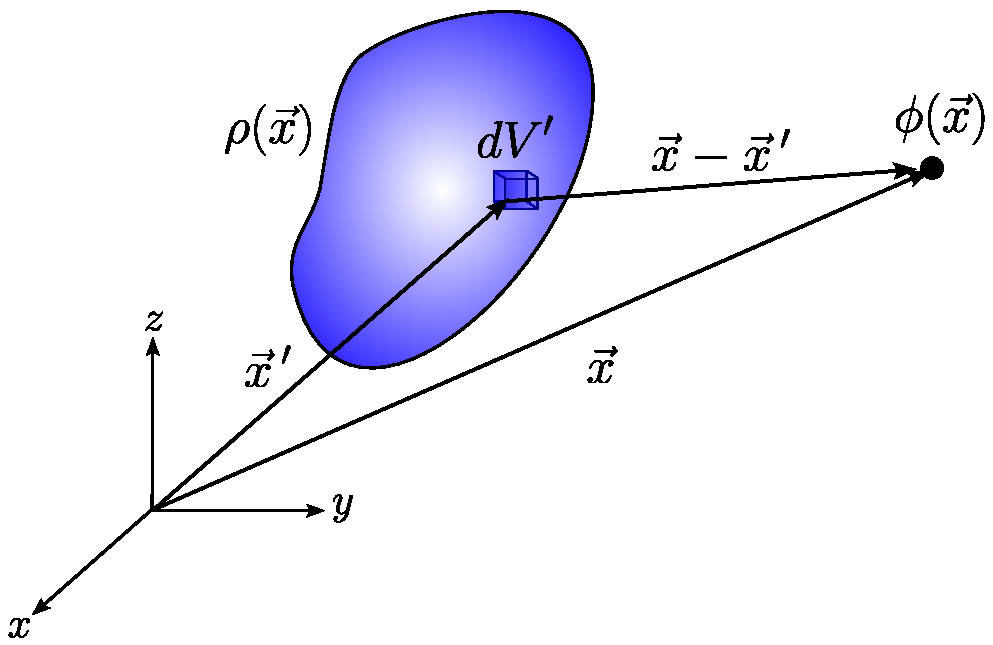
\includegraphics[width = 8cm]{Figuras/Distribucion-Cargas.pdf}
    \caption{Distribución de carga de densidad $\rho(\Vec{x})$.}
    \label{fig:PotencialDistribucion}
\end{figure}

Matemáticamente, podemos entender la convolución $f * g$ como \emph{el grado de traslape} entre dos pulsos, $f(y)$ y $g(-y)$, cuando uno $g(-y)$ se encuentra desplazado en $x$ unidades. Esta idea se puede observar en la figura \ref{fig:IdeaConvolucion}.

\begin{figure}[htbp]
    \centering
    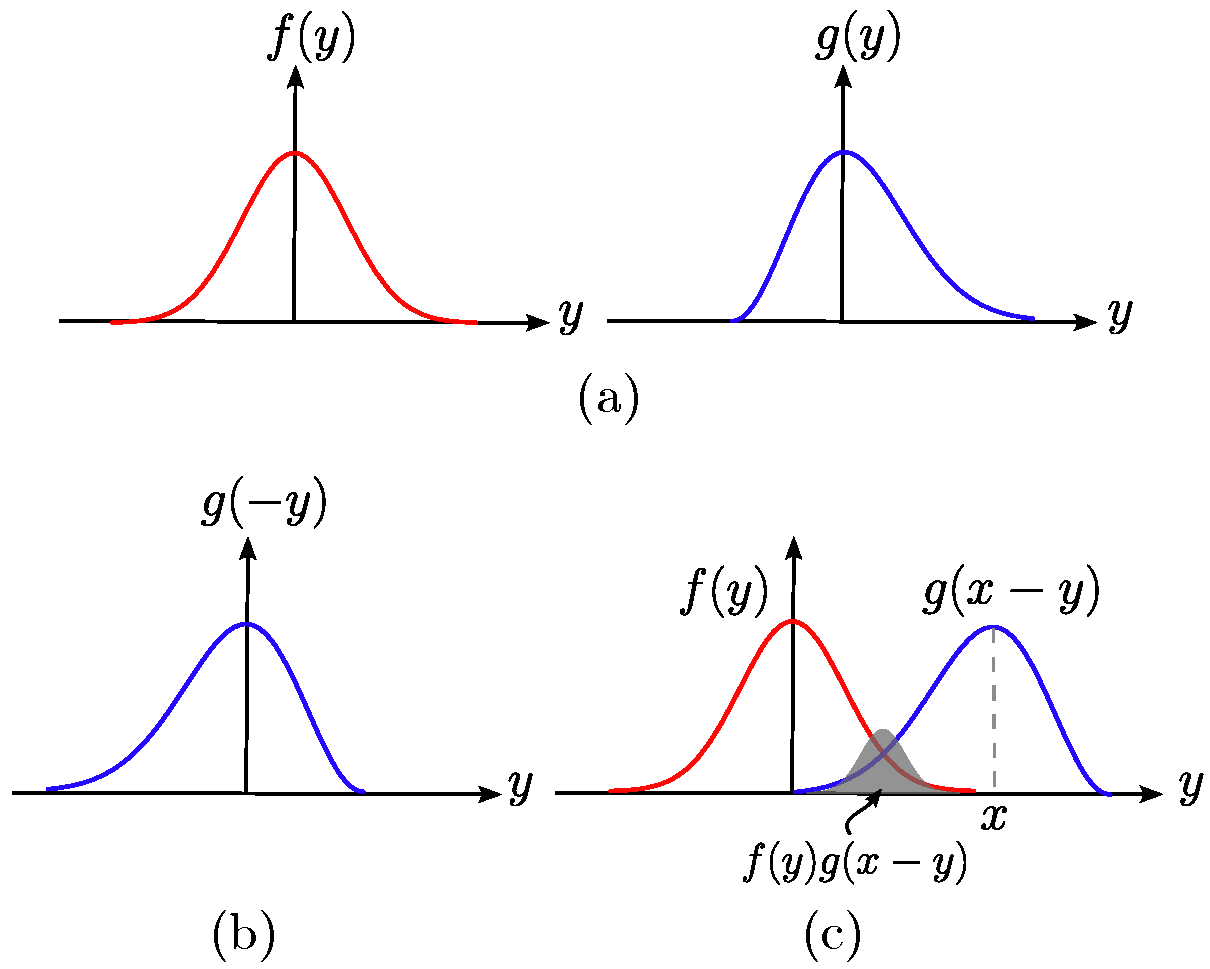
\includegraphics[width=10cm]{Figuras/Idea-Convolucion.pdf}
    \caption{Idea matemática de la convolución. En (a), se expresa cada función en términos de la variable de integración $y$. En (b), se refleja la gráfica de $g(y)$ con respecto al eje vertical, es decir, $g(y) \rightarrow g(-y)$. En (c), se traslada la gráfica de $g(-y)$, $x$ unidades. Luego, se traslapan las gráficas de $f(y)$ y $g(x-y)$ de tal forma que el área sombreada corresponde al valor de $f * g$ para ese valor de $x$.}
    \label{fig:IdeaConvolucion}
\end{figure}

% Entonces, $f * g$ mide el grado de traslape entre $f(y)$ y $g(-y)$, luego de trasladar $g$ a una distancia $x$.

\begin{propiedad}\textbf{Propiedades de la convolución.}

Sean $f(x)$, $g(x)$ y $h(x)$  funciones reales. Entonces, se verifican las siguientes propiedades:

\begin{enumerate}
    \item \textbf{Conmutatividad:}$$f(x) * g(x) = g(x) * f(x).$$
    
    \item \textbf{Asociatividad:} $$[f(x)*g(x)]*h(x) = f(x)*[g(x)*h(x)].$$
    
    \item \textbf{Distributividad:} $$f(x)*[g(x)+h(x)] = f(x)*g(x) + f(x)*h(x).$$ 
\end{enumerate}
\end{propiedad}

\newpage

\begin{teorema}[de convolución de Fourier]
Sean $f(x)$, $g(x)$ y $h(x)$  funciones reales y sean $\tilde{f}(k)$, $\tilde{g}(k)$ y $\tilde{h}(k)$ sus correspondientes transformadas de Fourier. 

\begin{itemize}
    \item Si $\tilde{h}(k) = \tilde{f}(k) \tilde{g}(k)$, entonces 
$$ h(x) = \frac{1}{\sqrt{2\pi}} (f * g)(x) = \frac{1}{\sqrt{2\pi}} \int_{-\infty}^{\infty} f(y) g(x-y) \,dy.$$ 

    \item Si $h(x) = f(x) g(x)$, entonces
    \begin{equation}
        \Tilde{h}(k) = \frac{1}{\sqrt{2\pi}}(\Tilde{f} * \Tilde{g})(k) = \frac{1}{\sqrt{2\pi}} \int_{-\infty}^{\infty} \Tilde{f}(y) \Tilde{g}(k-y) \,dy.
    \end{equation}
% $$$$
\end{itemize}
\end{teorema}

\begin{demo}
\ 

\begin{itemize}
    \item Supongamos que  $\tilde{h}(k) = \tilde{f}(k) \tilde{g}(k)$. Aplicando la transformada de Fourier inversa dada por \eqref{I.Fourier}, tenemos que 
\begin{align*}
   h(x) = \mathcal{F}^{-1} \{\tilde{h}(k)\} & = \mathcal{F}^{-1} \{\tilde{f}(k) \tilde{g}(k)\} \\
   & = \frac{1}{\sqrt{2\pi}} \int_{-\infty}^{\infty} \tilde{f}(k) \tilde{g}(k) e^{ikx} \,dk \\
   & = \frac{1}{\sqrt{2\pi}} \int_{-\infty}^{\infty}  \left( \frac{1}{\sqrt{2\pi}} \int_{-\infty}^{\infty} f(y) e^{-ik y} \,dy \right) \tilde{g}(k)  e^{ikx}  \,dk.
\end{align*}

Si el intercambio de orden de integración es posible, entonces 
\begin{align*}
  h(x) &= \frac{1}{\sqrt{2\pi}} \int_{-\infty}^{\infty}  f(y)  \left( \frac{1}{\sqrt{2\pi}} \int_{-\infty}^{\infty}  \tilde{g}(k)  e^{ikx} e^{-ik y}\,d k \right) \,dy \\
   & = \frac{1}{\sqrt{2\pi}} \int_{-\infty}^{\infty}  f(y)  \left( \frac{1}{\sqrt{2\pi}} \int_{-\infty}^{\infty}  \tilde{g}(k)  e^{ik(x-y)}\,d k \right) \,dy \\
   & = \frac{1}{\sqrt{2\pi}} \int_{-\infty}^{\infty}  f(y) g(x-y) \,dy = \frac{1}{\sqrt{2\pi}} (f * g)(x).
\end{align*}

Como la convolución es conmutativa:
$$h(x) = \frac{1}{2\pi} (f * g)(x) = \frac{1}{2\pi} (g * f)(x)  = \frac{1}{\sqrt{2\pi}} \int_{-\infty}^{\infty}  f(y) g(x-y) \,dy.$$

\item  Supongamos que $h(x) = f(x) g(x)$. Aplicando la transformada de Fourier dada por \eqref{T.Fourier}, tenemos que 
\begin{align*}
   \Tilde{h}(k) &=  \mathcal{F} \{f(x) g(x)\} \\
   &= \frac{1}{\sqrt{2\pi}} \int_{-\infty}^{\infty} f(x) g(x) e^{-ikx} \,dx \\
   &=  \frac{1}{\sqrt{2\pi}} \int_{-\infty}^{\infty} \left( \frac{1}{\sqrt{2\pi}} \int_{-\infty}^{\infty} \Tilde{f}(y) e^{iyx} \,dy \right) g(x) e^{-ikx} \,dx.
\end{align*}

Si el intercambio de orden de integración es posible, entonces 
\begin{align*}
   \Tilde{h}(k) &=  \frac{1}{\sqrt{2\pi}} \int_{-\infty}^{\infty} \Tilde{f}(y) \left( \frac{1}{\sqrt{2\pi}} \int_{-\infty}^{\infty} g(x) e^{iyx}  e^{-ikx}\,dx \right) \,dy \\
   &=  \frac{1}{\sqrt{2\pi}} \int_{-\infty}^{\infty} \Tilde{f}(y) \left( \frac{1}{\sqrt{2\pi}} \int_{-\infty}^{\infty} g(x) e^{-i(k-y)x} \,dx \right) \,dy \\
   &=  \frac{1}{\sqrt{2\pi}} \int_{-\infty}^{\infty} \Tilde{f}(y) \Tilde{g}(k-y) \,dy. 
\end{align*}

Por lo tanto,
$$\Tilde{h}(k) =  \frac{1}{\sqrt{2\pi}} (\Tilde{f} * \Tilde{g})(k) = \frac{1}{\sqrt{2\pi}} \int_{-\infty}^{\infty} \Tilde{f}(y) \Tilde{g}(k-y) \,dy.$$
\end{itemize}

\end{demo}


\begin{ejemplo}
    Sabiendo que \cite{Mauch}
    $$\mathcal{F}\left\{ \frac{2c}{x^2+c^2} \right\} = e^{-c|k|}, \quad \text{para} ~ c > 0.$$

    Podemos usar el teorema de convolución para encontrar la transformada de Fourier de
    \begin{equation}
      f(x) = \frac{1}{x^4+5x^2+4} = \frac{1}{(x^2+1)(x^2+4)}.    \label{EjConvo}
    \end{equation}
  
    En efecto,
    \begin{align*}
        \mathcal{F}\{f(x)\} &=  \mathcal{F}\left\{ \frac{1}{8} \frac{2}{x^2+1} \frac{4}{x^2+4} \right\} \\
        &= \frac{1}{8} \left( \int_{-\infty}^{\infty} e^{-|y|}e^{-2|k-y|} dy \right) \\
        &= \frac{1}{8} \left( \int_{-\infty}^0 e^{y}e^{-2|k-y|} dy +   \int_0^{\infty} e^{-y}e^{-2|k-y|} dy \right).
    \end{align*}

Si $k > 0$,
\begin{align*}
    \mathcal{F}\{f(x)\} &= \frac{1}{8} \left(  \int_{-\infty}^0 e^{y}e^{-2(k-y)} dy +  \int_0^k e^{-y}e^{-2(k-y)} dy + \int_k^{\infty} e^{-y}e^{2(k-y)} dy \right)  \\
    &= \frac{1}{8} \left(  \int_{-\infty}^0 e^{-2k+3y} dy +  \int_0^k e^{-2k+y} dy + \int_k^{+\infty} e^{2k-3y} dy \right) \\
    &= \frac{1}{8} \left( \frac{1}{3} e^{-2k} + e^{-k} - e^{-2k} + \frac{1}{3} e^{-k} \right) \\
    &= \frac{1}{6} e^{-k} - \frac{1}{12} e^{-2k}. 
\end{align*}

Si $k < 0$,
\begin{align*}
    \mathcal{F}\{f(x)\} &= \frac{1}{8} \left(  \int_{-\infty}^k e^{y}e^{-2(k-y)} dy +  \int_k^0 e^{y}e^{2(k-y)} dy + \int_0^{\infty} e^{-y}e^{2(k-y)} dy \right)  \\
    &= \frac{1}{8} \left(  \int_{-\infty}^k e^{-2k+3y} dy +  \int_k^0 e^{2k-y} dy + \int_0^{\infty} e^{2k-3y} dy \right) \\
    &= \frac{1}{8} \left( \frac{1}{3} e^{k} - e^{2k} + e^k + \frac{1}{3} e^{2k} \right) \\
    &= \frac{1}{6} e^{k} - \frac{1}{12} e^{2k}. 
\end{align*}

Por lo tanto, para $k$ positivo como negativo,
$$\boxed{\mathcal{F}\{f(x)\} =  \frac{1}{6} e^{-|k|} - \frac{1}{12} e^{-2|k|}} $$

Una mejor forma de encontrar la transformada de Fourier de \eqref{EjConvo} es, en primer lugar, descomponer la función en fracciones parciales,
$$f(x) = \frac{1}{3} \frac{1}{x^2+1} - \frac{1}{3} \frac{1}{x^2+4},$$

para luego hacer usar de la linealidad de la transformada.
\begin{align*}
     \mathcal{F}\{ f(x)\} &= \frac{1}{6} \mathcal{F} \left\{ \frac{2}{x^2+1}\right\} - \frac{1}{12} \mathcal{F} \left\{ \frac{4}{x^2+4} \right\}  \\
     &= \frac{1}{6} e^{-|k|} - \frac{1}{12} e^{-2|k|}.
\end{align*}

\end{ejemplo}

% \section{Aplicación de la transformada de Fourier}

% La transformada de Fourier es útil para resolver ecuaciones diferenciales en el dominio $(-\infty, \infty)$ con condiciones de borde homogéneas en el infinito. En particular, en ecuaciones diferenciales \underline{lineales} con \underline{coeficientes constantes}, debido a la propiedad de linealidad de la transformada.

% A continuación se ilustra el procedimiento a seguir mediante ejemplos.

% \begin{ejemplo}
%     Encuentre la solución general de la ecuación diferencial
%     $$y''(x) - y(x) = e^{-\alpha |x|}, \quad y(\pm \infty) = 0, \quad \alpha > 0, \alpha \neq 1.$$

%     \textbf{Solución:} La solución del caso homogéneo 
%     $$y''(x) - y(x) = 0,$$

%     está dada por
%     $$y_h(x) = c_1 e^{x} + c_2 e^{-x}, \quad c_1,c_2 \in \mathbb{R}.$$

%     Nos queda por encontrar la solución particular, para ello haremos uso de la transformada de Fourier. 

%     Primero, determinemos 
    
%     \begin{align*}
%         \mathcal{F}\left\{ e^{-\alpha |x|} \right\} &= \frac{1}{2\pi} \int_{-\infty}^{\infty} e^{-\alpha |x|} e^{-ikx} dx \\
%         &= \frac{1}{2\pi} \left(  \int_{-\infty}^{0} e^{x(\alpha -ikx)} dx +  \int_{0}^{\infty} e^{-x(\alpha + ik)} dx\right) \\
%         &= \frac{1}{2\pi} \left( \frac{1}{\alpha -ik} + \frac{1}{\alpha +ik} \right) \\
%         &= \frac{\alpha/\pi}{\alpha^2 + k^2}.
%     \end{align*}

%     Luego, apliquemos la transformada de Fourier a la ecuación diferencial:
%     \begin{align*}
%         \mathcal{F}\{ y''(x)\} - \mathcal{F}\{y(x)\ &=  \mathcal{F}\left\{ e^{-\alpha |x|} \right\} \\
%         \Rightarrow - k^2 \mathcal{F}\{y(x)\} - \mathcal{F}\{y(x)\} &= \frac{\alpha/\pi}{\alpha^2 + k^2}.
%     \end{align*}

%     Despejando la transformada de Fourier de la solución.
%     \begin{align*}
%         \mathcal{F}\{y(x)\} &= \frac{-\alpha/\pi}{(k^2 + \alpha^2)(k^2+1)} \\
%         &= - \frac{\alpha}{\pi} \frac{1}{\alpha^2-1} \left( \frac{1}{k^2+1} - \frac{1}{k^2+ \alpha^2}\right) \\
%         &= \frac{1}{\alpha^2-1} \left( \frac{\alpha/\pi}{k^2 + \alpha^2} - \alpha \frac{1/\pi}{k^2+1} \right.)
%     \end{align*}

%     Tomando la transformada inversa, obtenemos que
%     $$y(x) = \frac{e^{-\alpha|x| - \alpha e^{-|x|} }}{\alpha^2-1}.$$

%     Por lo tanto, la solución general es
%     $$\boxed{y(x) = \frac{e^{-\alpha|x| - \alpha e^{-|x|} }}{\alpha^2-1} + c_1 e^{x} + c_2 e^{-x}, \quad c_1,c_2 \in \mathbb{R}}$$
% \end{ejemplo}

% \begin{ejemplo}
%   Consideremos un oscilador armónico amortiguado sometido a una fuerza externa $g(t)$. La ecuación de movimiento del oscilador está dada por
% \begin{equation}
%  \ddot{x}(t) + 2 \alpha \dot{x}(t) + \omega_0^2 x(t) = f(t), \label{EDO-Oscilador}   
% \end{equation}

% donde $f(t) = g(t)/m$ y $\alpha$ es una constante asociada al amortiguamiento del sistema. En los primeros cursos de Ecuaciones Diferenciales Ordinarias (EDO) se trabaja con $f(t)$ sinusoidal, pero gracias a la transformada de Fourier, podemos extender este resultado para funciones $f(t)$ arbitrarias. 

% Aplicando la transformada de Fourier en la variable temporal, a saber,
% $$\mathcal{F}\{x(t)\} = \frac{1}{2\pi} \int_{-\infty}^{\infty} f(t) e^{-i\omega t} dt, $$

% a ambos lados de la ecuación diferencial \eqref{EDO-Oscilador}, obtenemos 
% \begin{align}
%     \mathcal{F}\left\{ \ddot{x}(t) + 2 \alpha \dot{x}(t) + \omega_0^2 x(t)\right\} &= \mathcal{F}\left\{ f(t)\right\} \nonumber\\
%     \Rightarrow   \mathcal{F}\left\{ \ddot{x}(t) \right\} + 2\alpha \mathcal{F}\left\{ \dot{x}(t) \right\} + \omega_0^2 \mathcal{F}\{x(t)\} &= \mathcal{F}\left\{ f(t)\right\}. \label{EDO-Transformada}
% \end{align}

% Si asumimos que 
% $$\lim_{x \to \pm \infty} x(t) = \lim_{x \to \pm \infty} \dot{x}(t) = 0,$$

% tenemos 
% \begin{align*}
%      \mathcal{F}\left\{ \ddot{x}(t) \right\} &= (i\omega)^2 \mathcal{F}\{x(t)\} = - \omega^2 \mathcal{F}\{x(t)\},\\
%       \mathcal{F}\left\{ \dot{x}(t) \right\} &= i \omega \mathcal{F}\{x(t)\}.
% \end{align*}

% Además, si definimos $F(\omega) := \mathcal{F}\left\{ f(t)\right\}$, la ecuación \eqref{EDO-Transformada} nos queda
% $$ - \omega^2 \mathcal{F}\{x(t)\} + 2 \alpha \omega i \mathcal{F}\{x(t)\} + \omega_0^2 \mathcal{F}\{x(t)\} = F(\omega).$$

% Despejando la transformada de Fourier de la solución:
% $$  \mathcal{F}\{x(t)\} = \frac{F(\omega)}{-\omega^2 - 2 \alpha i \omega + \omega_0^2}.$$

% Tomando la transformada inversa, obtenemos la solución 
% $$\boxed{x(t) = \int_{-\infty}^{\infty} \frac{F(\omega)}{(\omega_0^2-\omega^2) - 2 \alpha \omega i} e^{i\omega t} d\omega }$$  
% \end{ejemplo}